\documentclass[border=10pt]{standalone}
\ifdefined\pdfoutput
    \ifnum\pdfoutput>0
        % PDF mode
    \else
        \def\pgfsysdriver{pgfsys-dvisvgm.def}
    \fi
\else
    \def\pgfsysdriver{pgfsys-dvisvgm.def}
\fi
\usepackage{tikz}
\usetikzlibrary{shapes.geometric, arrows.meta, positioning, calc}
\usepackage{xcolor}

\begin{document}
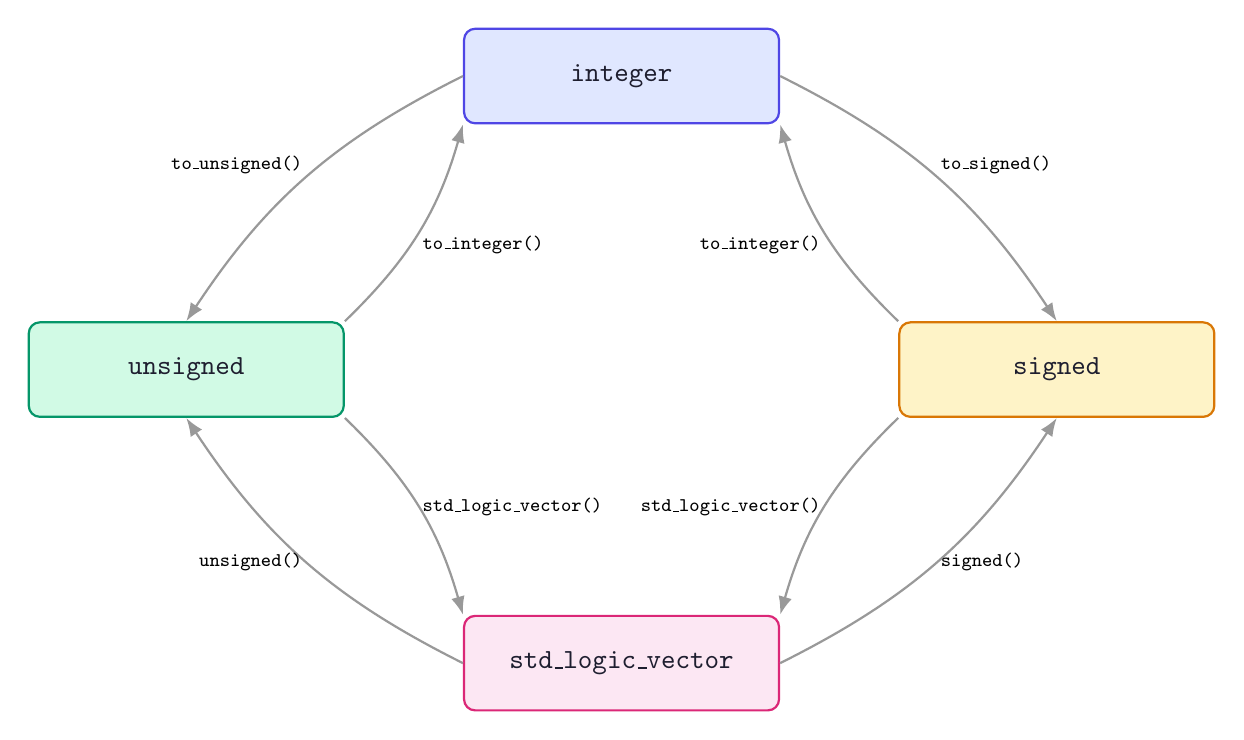
\begin{tikzpicture}[
    >=Latex,
    node distance=2.5cm and 3cm,
    font=\sffamily
]

\definecolor{colorint}{HTML}{E0E7FF}
\definecolor{borderint}{HTML}{4F46E5}

\definecolor{colorus}{HTML}{D1FAE5}
\definecolor{borderus}{HTML}{059669}

\definecolor{colors}{HTML}{FEF3C7}
\definecolor{borders}{HTML}{D97706}

\definecolor{colorslv}{HTML}{FCE7F3}
\definecolor{borderslv}{HTML}{DB2777}

\definecolor{mytext}{HTML}{1E1E2F}

\tikzset{
    typebase/.style={
        rectangle, 
        rounded corners, 
        thick,
        minimum width=4cm,
        minimum height=1.2cm,
        text=mytext,
        font=\ttfamily\bfseries,
        align=center
    },
    arr/.style={
        ->, 
        thick, 
        draw=gray!80,
        text=black,
        font=\ttfamily\scriptsize
    }
}

% Nodes
\node[typebase, draw=borderint, fill=colorint] (int) {integer};
\node[typebase, draw=borderus, fill=colorus, below left=2.5cm and 1.5cm of int] (us) {unsigned};
\node[typebase, draw=borders, fill=colors, below right=2.5cm and 1.5cm of int] (s) {signed};
\node[typebase, draw=borderslv, fill=colorslv, below right=2.5cm and 1.5cm of us] (slv) {std\_logic\_vector};

% Edges between integer and unsigned
\draw[arr] (int.west) to[bend right=15] node[above left, inner sep=1pt] {to\_unsigned()} (us.north);
\draw[arr] (us.north east) to[bend right=15] node[below right, inner sep=1pt] {to\_integer()} (int.south west);

% Edges between integer and signed
\draw[arr] (int.east) to[bend left=15] node[above right, inner sep=1pt] {to\_signed()} (s.north);
\draw[arr] (s.north west) to[bend left=15] node[below left, inner sep=1pt] {to\_integer()} (int.south east);

% Edges between unsigned and std_logic_vector
\draw[arr] (us.south east) to[bend left=15] node[right, inner sep=1pt] {std\_logic\_vector()} (slv.north west);
\draw[arr] (slv.west) to[bend left=15] node[left, inner sep=1pt] {unsigned()} (us.south);

% Edges between signed and std_logic_vector
\draw[arr] (s.south west) to[bend right=15] node[left, inner sep=1pt] {std\_logic\_vector()} (slv.north east);
\draw[arr] (slv.east) to[bend right=15] node[right, inner sep=1pt] {signed()} (s.south);

\end{tikzpicture}
\end{document}
